\section{Profiling Infrastructure}
Our profiling framework comprises three parts:

\begin{itemize}
\item Support in GHC's runtime for tracing events to a log file at
  runtime.  The tracing is designed to be as lightweight as possible,
  so as not to have any significant impact on the behaviour of the
  program being measured.

\item A Haskell library \codef{ghc-events} that can read the trace file
  generated by the runtime and build a Haskell data structure
  representing the trace.

\item Multiple tools make use of the \codef{ghc-events} library to read and
  analyze trace files.
\end{itemize}

Having a single trace-file format and a library that parses it means
that it is easy to write a new tool that works with GHC trace files:
just import the \codef{ghc-events} package and write code that uses the
Haskell data structures directly.  We have already built several such
tools ourselves, some of which are merely proof-of-concept
experiments, but the \codef{ghc-events} library makes it almost trivial to
create new tools:

\begin{itemize}
\item A simple program that just prints out the (sorted) contents of
  the trace file as text.  Useful for checking that a trace file can
  be parsed, and for examining the exact sequence of events.

\item The ThreadScope graphical viewer.

\item A tool that parses a trace file and generates a PDF format
  timeline view, similar to the ThreadScope view.

\item A tool that generates input in the format expected by the
  GtkWave circuit waveform viewer.  This was used as an early
  prototype for ThreadScope, since the timeline view that we want to
  display has a lot in common with the waveform diagrams that gtkwave
  displays and browses.
\end{itemize}

\subsection{Fast runtime tracing}
Minimizing the overhead of event logging is critical when designing a system
to facilitate runtime tracing.  In the GHC runtime, a pre-allocated events buffer is 
used by each HEC to store generated events.
By doing so, we prevent any performance delays from dynamic 
memory allocation, and require no locks since the buffers are
HEC-local.  Yet, this requires us to flush the buffer
to the filesystem once it becomes full, but since the buffer is a
fixed size we pay a near-constant penalty for each flush and a
deterministic delay on the GHC runtime.

The HEC-local buffers are flushed independently, which means that
events in the log file appear out-of-order and have to be sorted.
Sorting of the events is easily performed by the profiling tool after
reading in the log file using the \codef{ghc-events} library.

To measure the speed at which the GHC runtime can log events, we used
a C program (no Haskell code, just using the GHC runtime system as a
library) that simply generates 2,000,000 events, alternating between
``thread start'' and ``thread stop'' events.  Our program generates a
34MB trace file and runs in 0.31 seconds elapsed time:

\begin{figure*}
\begin{center}
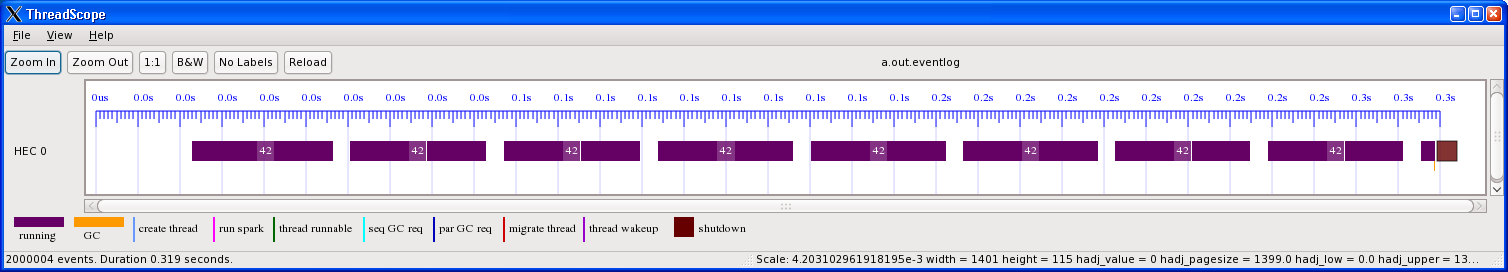
\includegraphics[scale=0.3]{eventbench.png}
\end{center}
\caption{Synthetic event benchmark}
\label{f:event-bench}
\end{figure*}

\begin{verbatim}
  INIT  time    0.00s  (  0.02s elapsed)
  MUT   time    0.22s  (  0.29s elapsed)
  GC    time    0.00s  (  0.00s elapsed)
  EXIT  time    0.00s  (  0.00s elapsed)
  Total time    0.22s  (  0.31s elapsed)
\end{verbatim}
which gives a rough figure of 150ns for each event on average.
Looking at the ThreadScope view of this program
(Figure~\ref{f:event-bench}) we can clearly see where the buffer
flushes are happening, and that each one is about 5ms long.

An alternative approach is to use memory-mapped files, and write our
events directly into memory, leaving the actual file writing to the
OS.  This would allow writing to be performed asynchronously, which
would hopefully reduce the impact of the buffer flush.  According to
\codef{strace} on Linux, the above test program is spending 0.7s
writing buffers, so making this asynchronous would save us about 30ns
per event on average.  However, on a 32-bit machine where we can't
afford to reserve a large amount of address space for the whole log
file, we would still have to occasionally flush and remap new portions
of the file.  This alternative approach is something we plan to
explore in the future.

% how much impact does this have on runtimes?
To see how much impact event logging has on real execution times, we
took a parallel version of the canonical Fibonacci function,
\codef{parfib}, and compared the time elapsed with and without event
logging enabled for 50 executions of parfib on an Intel(R) Core(TM)2
Duo CPU T5250 1.50GHz, using both cores.  The program generates about
2,000,000 events during the run, and generates a 40MB log file.

\begin{verbatim}
  parfib eventlog 
  ./Main 40 10 +RTS -N2 -l -RTS
  Avg Time Elapsed  Standard Deviation
  20.582757s        0.789547s

  parfib without eventlog 
  ./Main 40 10 +RTS -N2 -RTS
  Avg Time Elapsed  Standard Deviation
  17.447493s        1.352686s
\end{verbatim}

Considering the significant number of events generated in the traces
and the very detailed profiling information made available by these
traces, the overhead does not have an immense impact at approximately
10-25\% increase in elapsed time.  In the case of parfib, the event
representing the creation of a new spark is dominant, comprising at
least 80\% of the the events generated.  In fact, it is debatable
whether we should be logging the creation of a spark, since the cost
of logging this event is likely to be larger than the cost of creating
the spark itself - a spark creation is simply a write into a circular
buffer.
  
For parallel quicksort, far fewer sparks are created and most of the
computation is spent in garbage collection; thus, we can achieve an
almost unnoticeable overhead from event tracing.  The parallel quicksort
example involved sorting a list of 100,000 randomly generated integers
and was performed in the same manner as parfib where we compare with
event logging and without, yet in this test we perform 100 executions 
on an Intel(R) Core(TM) 2 Quad CPU 3.0Ghz. 

\begin{verbatim}
  parquicksort eventlog 
  ./Main +RTS -N4 -l -RTS 
  Avg Time Elapsed  Standard Deviation
  14.201385s        2.954869

  parquicksort without eventlog 
  ./Main +RTS -N4 -RTS 
  Avg Time Elapsed  Standard Deviation
  15.187529s        3.385293s

\end{verbatim}

Since parallel quicksort spent the majority of the computation doing
useful work, particularly garbage collection of the created lists, a
trace file of only approximately 5MB and near 300,000 events was
created and the overhead of event tracing is not noticeable.

The crux of the event tracing is that even when a poorly performing
program utilizes event tracing, the overhead should still not be
devastating to the program's performance, but best of all on a program
with high utilization event tracing should barely affect the performance.

\subsection{An extensible file format}

We believe it is essential that the trace file format is both
backwards and forwards compatible, and architecture independent.  In
particular, this means that:

\begin{itemize}
\item If you build a newer version of a tool, it will still work with
  the trace files you already have, and trace files generated by
  programs compiled with older versions of GHC.

\item If you upgrade your GHC and recompile your programs, the trace
  files will still work with any profiling tools you already have.

\item Trace files do not have a shelf life.  You can keep your trace
  files around, safe in the knowledge that they will work with future
  versions of profiling tools.  Trace files can be archived, and
  shared between machines.
\end{itemize}

Nevertheless, we don't expect the form of trace files to remain
completely static.  In the future we will certainly want to add new
events, and add more information to existing events.  We therefore
need an extensible file format.  Informally, our trace files are
structured as follows:

\begin{itemize}
\item A list of \emph{event types}.  An event-type is a
  variable-length structure that describes one kind of event.  The
  event-type structure contains
  \begin{itemize}
    \item A unique number for this event type
    \item A field describing the length in bytes of an instance of the
      event, or zero for a variable-length event.
    \item A variable-length string (preceded by its length) describing
      this event (for example ``thread created'')
    \item A variable-length field (preceded by its length) for future
      expansion.  We might in the future want to add more fields to
      the event-type structure, and this field allows for that.
  \end{itemize}
\item A list of \emph{events}.  Each event begins with an event number
  that corresponds to one of the event types defined earlier, and the
  length of the event structure is given by the event type (or it has
  variable length).  The event also contains
  \begin{itemize}
  \item A nanosecond-resolution timestamp.
  \item For a variable-length event, the length of the event.
  \item Information specific to this event, for example which CPU it
    occurred on.  If the parser knows about this event, then it can
    parse the rest of the event's information, otherwise it can skip
    over this field because its length is known.
  \end{itemize}
\end{itemize}

The unique numbers that identify events are shared knowledge between
GHC and the \codef{ghc-events} library.  When creating a new event, a new
unique identifier is chosen; identifiers can never be re-used.

Even when parsing a trace file that contains new events, the parser
can still give a timestamp and a description of the unknown events.
The parser might encounter an event-type that it knows about, but the
event-type might contain new unknown fields.  The parser can recognize
this situation and skip over the extra fields, because it knows the
length of the event from the event-type structure.  Therefore when a
tool encounters a new log file it can continue to provide consistent
functionality.

Of course, there are scenarios in which it isn't possible to provide
this ideal graceful degradation.  For example, we might construct a
tool that profiles a particular aspect of the behaviour of the
runtime, and in the future the runtime might be redesigned to behave
in a completely different way, with a new set of events.  The old
events simply won't be generated any more, and the old tool won't be
able to display anything useful with the new trace files.  Still, we
expect that our extensible trace file format will allows us to smooth
over the majority of forwards- and backwards-compatibility issues that
will arise between versions of the tools and GHC runtime.  Moreover,
extensibility costs almost nothing, since the extra fields are all in
the event-types header, which has a fixed size for a given version of
GHC.
